\mbchapter{Performance von Webanwendungen}
Der Begriff Performance wurde in einschlägigen literarischen Werken bereits ausgiebig diskutiert. Die folgende Definition soll daher in dieser Arbeit als Basis herangezogen werden \cite{Smith2001}: 
\begin{quote}
"Performance is the degree to which a software system or component meets its objectives for timeliness“. 
\end{quote}
Mit \glqq timeliness\grqq{} ist dabei das Antwortzeitverhalten, also die Geschwindigkeit des Systems aus Sicht des Anwenders gemeint. Das Antwortzeitverhalten ist ein wichtiger Aspekt für die Beurteilung der Qualität des Softwaresystems durch den Anwender. Verzögerungen bei der Eingabe oder lange Wartezeiten wirken sich demnach negativ auf das Anwenderempfinden aus. Eine Studie der Firma Apigee hat gezeigt, dass 44\% aller Anwender Apps aufgrund mangelnder Performance sofort deinstallieren \cite{APIGEE}. Neben anderen Aspekten ist es für den Erfolg einer App demnach wichtig, ein gutes Antwortzeitverhalten vorzuweisen.

\section{Kategorien von Performance-Problemen}
\label{performance-kategorien}
Ein schlechtes Antwortzeitverhalten kann viele Ursachen haben. Die Codecentric AG hat in diesem Zusammenhang auf Basis von Großprojekten und Performance-Analysen acht allgemeine Kategorien von Ursachen schlechter Performance erarbeitet (Tabelle \ref{table-cc-performance})\cite{cc-performance}. Diese allgemeinen Kategorien sollen in dieser Arbeit für \gls{sp} Anwendungen konkretisiert werden. Dafür ist jedoch zunächst ein tieferes Verständnis der Funktionsweise dieser Anwendungen und von Browser-Engines erforderlich. Aus diesem Grund wird in den folgenden Abschnitten zunächst die Funktionsweise einer Browser-Engine analysiert, um anschließend diese Kategorien auf \gls{sp} Anwendungen zu übertragen. 
\begin{table}
	\centering
	\begin{tabular}{lp{8cm}}
	\textbf{Problemkategorien} & \textbf{Beschreibung}\\
	\hline
	Ineffiziente Algorithmen & Es kommt schon bei geringer Last zu schlechtem Antwortzeitverhalten, weil umständliche Algorithmen implementiert wurden.\\
	Ineffiziente Zugriffspfade & Ein Spezialfall ineffizienter Algorithmen, bei dem der Datenspeicher eine suboptimale Lösung für die Durchführung einer Datenabfrage ermittelt.\\
	Speicherleck\\(engl. "memory leak") & Es kommt zu einer Verschlechterung des Antwortzeitverhaltens bei längeren Laufzeiten, verursacht durch mangelhaftes Speichermanagement.\\
	Reinitialisierungsproblem & Das System verhält sich bei zunehmender Last unberechenbar, weil Speicherbereiche vor der Verwendung nicht sauber initialisiert werden.\\
	Flaschenhälse & Es kommt zu exponentiell steigenden Antwortzeiten, weil an bestimmten Systemstellen eine Warteschlange entsteht. Dabei werden pro Zeiteinheit mehr Anfragen an die Systemstelle herangetragen als verarbeitet werden können.\\
	Intermittierende Probleme & Das System reagiert plötzlich mit sehr schlechten Antwortzeiten, weil zum Beispiel die Netzwerkverfügbarkeit durch andere Prozesse gestört ist.\\
	Ressourcenauslastung & Es kommt zu einer exponentiellen Verschlechterung des Antwortzeitverhaltens bei Erhöhung der Last, weil sich die CPU-Auslastung an bestimmten Systemknoten der Auslastungsgrenze nähert.\\
	\end{tabular}
	\caption{Kategorien von Performance Problemen \cite{cc-performance}}
	\label{table-cc-performance}
\end{table}

\newpage
\section{Browser-Engines}
\label{browser-engines}
Der konkrete Ablauf in einem Browser hängt von der jeweiligen Implementierung ab. Jeder Browser funktioniert hier etwas anders. Dennoch sind grundlegende Abläufe und Strukturen meist gleich und zum Teil auch durch Standards definiert\cite{DOMTR}\cite{HTML-Parsing}. Eine grobe Betrachtung der Abläufe ist daher ohne Fokussierung auf einen speziellen Browser möglich. 
\\\\
Als Grundlage dieser Betrachtung wird eine Zusammenfassung der Funktionsweise aktueller Browser von Tali Garsiel herangezogen. Sie hat über einige Jahre Implementierungen von Oben-Source Browsern analysiert und ihre Erkenntnisse zusammengefasst\cite{hbw}.
\\\\
Ein Browser besteht demnach aus den in Abbildung \ref{hbw-ebenen} dargestellten Komponenten. Das \gls{ui} stellt dem Anwender alle Komponenten für die Interaktion mit der Webseite zur Verfügung. Ein Beispiel dafür sind die Vor-/Zurück-Schaltflächen oder Lesezeichen. Eine Ebene tiefer befindet sich die Browser-Engine. Sie dient als Schnittstelle zwischen dem User Interface und der Rendering Engine. Der wichtigste Bestandteil ist die Rendering-Engine. Sie ist für die Anzeige von \gls{html}-Dateien zuständig und kommuniziert dabei mit einem JavaScript Interpreter und einer Netzwerkschnittstelle. Ein Beispiel für eine Rendering Engine ist WebKit in Safari oder Blink in Chrome und Opera.\cite{Blink}\cite{WebKit}
\begin{figure}[h]
	\centering
	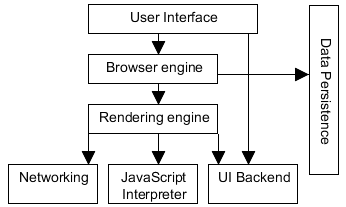
\includegraphics[scale=0.8]{Bilder/Browser-Layout.png}
	\caption{Schichten eines Browsers \cite{hbw}}
	\label{hbw-ebenen}
\end{figure}
Für das Anzeigen einer URL ruft die Rendering Engine zunächst die \gls{html}-Datei von der Netzwerkschnittstelle ab. Diese Schnittstelle liefert das Dokument in Blöcken und die Rendering-Engine beginnt mit der Verarbeitung. Zu Beginn wird die \gls{html}-Datei interpretiert und in einzelne Elemente aufgeteilt. Aus diesen Elementen entsteht das \gls{dom}, auch \gls{dom}-Tree genannt. Verweise auf \gls{css}-Dateien werden aufgelöst und sobald möglich ebenfalls interpretiert. Es entstehen weitere Elemente die das \gls{cssom}, auch \gls{cssom}-Tree genannt, bilden. Beide Trees werden im nächsten Schritt zu einem Render-Tree zusammengefasst. Er enthält nur sichtbare Elemente inklusive ihrer Formatierungseigenschaften. Durch den Layout-Prozess erhält anschließend jedes Element des Render-Tree eine feste Position auf dem Bildschirm und kann dadurch im letzten Schritt gezeichnet werden (Abbildung \ref{hbw-flow}).\cite{hbw}\cite{g-rendertree}
\begin{figure}[h]
	\centering
	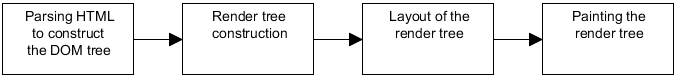
\includegraphics[scale=0.8]{Bilder/Browser-Engine-Flow.png}
	\caption{Workflow eines Browsers \cite{hbw}}
	\label{hbw-flow}
\end{figure}
\\\\
Das Parsen eines \gls{html}-Dokumentes kann bereits durchgeführt werden, wenn erste Teile des Dokumentes über die Netzwerkschnittstelle eingetroffen sind. Dadurch verkürzt sich die Wartezeit für den Anwender\cite{hbw}. Problematisch wird es, wenn JavaScript-Verweise in einem Dokument vorhanden sind. Prinzipiell verzögert sich dadurch das Parsen und damit auch die schnelle Anzeige des Dokumentes. Denn JavaScript wird ausgeführt, sobald es beim Parsen gefunden wird \cite[S. 1]{Zakas2010}. 
\\\\ 
Externe Ressourcen (JavaScript, \gls{css}, Bilder, etc.) werden beim Parsen über die Netzwerkschnittstelle heruntergeladen. Um diesen Vorgang zu beschleunigen, öffnen die verschiedenen Browser eine unterschiedliche Anzahl paralleler Verbindungen. In Chromium werden beispielsweise maximal 6 parallele Verbindungen zugelassen \cite{ss-parallelconnections}. Befinden sich mehr externe Ressourcen in einem Dokument, verzögert sich demnach das Herunterladen und Ausführen, bis  freie Verbindungen vorhanden sind. Zu dieser Problematik zählen auch Abfragen über \gls{xhr}.
\\\\
Der Begriff \gls{sp} Anwendung beschreibt in Bezug auf Webtechnologien eine Website, die aus einer einzigen \gls{html}-Datei besteht. Der Inhalt dieser Datei ändert sich dynamisch zur Laufzeit der Anwendung \cite{jp-spm}. Bei dieser Art von Anwendung fällt Schritt 1 in Abbildung \ref{hbw-flow} nur beim ersten Aufruf der Website ins Gewicht. Der \gls{dom}- und \gls{cssom}-Tree wird nur einmalig erstellt und während der Laufzeit der Anwendung lediglich geändert. Durch Aktionen in JavaScript kann auf den \gls{dom} zugegriffen werden. Das Abfragen oder Setzen von Werten in einem \gls{dom}-Element oder das Entfernen und Hinzufügen neuer \gls{dom}-Elemente kann den Effekt haben, dass die Rendering-Engine einen \gls{Reflow} durchführen muss. Der Begriff \gls{Reflow} bezeichnet die Neuberechnung der Positionen und das Zeichnen aller Elemente. In Abbildung \ref{hbw-flow} bezeichnet dies die Schritte drei und vier. \glspl{Reflow} sind aufgrund des Single-Thread Models von JavaScript blockierend und sollten daher vermieden werden \cite{dg-reflow}. Kritisch für die Performance einer \gls{sp} Anwendung ist demnach das Layouten und Rendern, sowie die generelle JavaScript Ausführung. 
\\\\
Im Hinblick auf die Performance lassen sich aus diesen Vorgängen bereits grundlegende Regeln ableiten: 
\begin{itemize}
	\item Die Größe des \gls{html}-Dokument bestimmt die Zeit für das Erstellen des \gls{dom}-Tree.
	\item Die Anzahl der \gls{css}- und JavaScript-Verweise beeinflusst die Zeit für das Erstellen des \gls{dom}-Tree.
	\item Die Anzahl der \gls{css}-Regeln und deren Komplexität bestimmt die Zeit für die Erstellung des \gls{cssom}-Tree. 
	\item Die Größe des \gls{dom}- und \gls{cssom}-Tree bestimmen die Zeit für das Erstellen des Render-Tree.
	\item Die Anzahl der Elemente im Render-Tree bestimmt die Zeit für das Layouten.
	\item Die Anzahl der Elemente im Render-Tree bestimmt die Zeit für das Zeichnen.
	\item Die Komplexität des \gls{html}/\gls{css} beeinflusst demnach das Antwortzeitverhalten.
	\item Das Management externer Ressourcen beeinflusst ebenfalls das Antwortzeitverhalten.
\end{itemize}

\section{Kategorien im Web}
\label{performance-categories-web}

In diesem Abschnitt werden die zuvor genannten Kategorien auf \gls{sp} Anwendungen übertragen. Im Ergebnis ergeben sich generelle Schwachstellen, die in den folgenden Kapiteln berücksichtigt werden müssen und schon erste Erkenntnisse für das Ergebnis dieser Arbeit darstellen. Zum Vergleich mit den allgemeinen Kategorien kann die Tabelle \ref{table-cc-performance} herangezogen werden.
\\\\
\textbf{Ineffiziente Algorithmen}
\\
Dieses Problem hat wenig mit der verwendeten Technologie zu tun. Denn egal in welcher Sprache, langsame Algorithmen können immer der Grund für eine schlechte Performance sein.  Analysen oder Code-Reviews können solche Probleme bereits im Vorfeld vermeiden.
\\\\
\textbf{Ineffiziente Zugriffspfade}
\\
Der Zugriff auf einen Datenspeicher wird auf eine langsame Art und Weise durchgeführt. In Bezug auf JavaScript tritt dieses Problem beim Zugriff auf klassische Speichermöglichkeiten wie den Session- oder \gls{LocalStorage} auf. Jedoch auch der \gls{dom} als persistenter Speicher für den aktuellen Status der View fällt in diese Kategorie. Wie in Abschnitt \ref{browser-engines} beschrieben, können Zugriffe auf Elemente im \gls{dom} einen \gls{Reflow} auslösen. Dies wirkt sich entsprechend negativ auf die Performance aus. Daher ist bei solch einem Zugriff immer darauf zu achten, auf welche Attribute der Zugriff erfolgt. 
\\\\
\textbf{Speicherleck (engl. \glqq memory leak\grqq)}
\\
Unter einem Speicherleck versteht man einen Bereich bzw. ein Objekt im Speicher, zu dem es keine Referenz mehr gibt. In JavaScript soll sich der \gls{gc}, um das Freigeben solcher Bereiche kümmern. Dennoch kann es auch in heutigen Browsern noch vorkommen, dass es dem \gls{gc} nicht möglich ist festzustellen, ob noch Referenzen auf ein Objekt vorhanden sind und es daher freigeben werden muss. Speicherlecks sorgen dafür, dass die Speicherauslastung zur Laufzeit der Anwendung  immer weiter ansteigt. Im Ergebnis friert eine Anwendung ein, wenn die Speicherauslastung zu hoch ist. Relevant ist dies nur bei Anwendungen, die über eine lange Zeit genutzt werden. Herkömmliche Webseiten, also Anwendungen mit häufigen \gls{PageReloads}, hatten hingegen meist eine kurze Laufzeit und waren dadurch nicht von diesem Problem betroffen. Spätestens beim Schließen der Seite wurde der gesamte verwendete Speicher freigegeben. Im Hinblick auf \gls{sp} Anwendungen ist dies jedoch ein größeres Problem. Durch das dynamische Ändern der Seite, im Gegensatz zum Aufrufen einer neuen Seite, haben \gls{sp} Anwendungen meist eine lange Laufzeit. Gelangt man mit solch einer Anwendung an die Grenzen des verfügbaren Speichers, wird der \gls{gc} zunehmend aktiv, was sich negativ auf das Antwortzeitverhalten auswirkt. Außerdem können dynamische Inhalte nicht erstellt werden, wenn der Arbeitsspeicher vollständig belegt ist.\cite{JSMemoryLeaks1}\cite{JSMemoryLeaks2}
\\\\
\textbf{Reinitialisierungsproblem}\\Dieses Problem bezieht sich auf die Verwendung von Variablen, die nicht initialisiert wurden. Aufgrund von daraus resultierenden Fehlern können Probleme mit der Performance entstehen. Bei Programmiersprachen ohne automatische Speicherverwaltung wie C++ haben solche Variablen einen Wert, der dem entspricht, was sich zuletzt an der jeweiligen Speicheradresse befunden hat. Eine Verwendung dieses Wertes kann Laufzeitfehler verursachen. Unter JavaScript spielt dieses Problem keine Rolle, da neue Variablen standardmäßig mit dem Wert \emph{undefined} initialisiert werden \cite[S. 41ff.]{Flanagan2011}.
\\\\
\textbf{Flaschenhälse}
\\
Flaschenhälse sind Komponenten einer Anwendung, die durch Anfragen so sehr belastet werden, dass Warteschlangen entstehen. Der Zugriff auf diese Komponenten dauert entsprechend lange. In JavaScript gehört der asynchrone \gls{xhr}-Zugriff in diese Kategorie. Wie in Abschnitt \ref{browser-engines} beschrieben, öffnet jeder Browser nur eine maximale Anzahl paralleler Verbindungen. Werden mehr Anfragen gestellt als Antworten eintreffen, bildet sich eine Warteschlange und das Antwortzeitverhalten verschlechtert sich.
\\\\
Ein weiteres Problem in dieser Kategorie ist das Single-Thread Model von JavaScript. Lange Algorithmen oder synchrone \gls{xhr}-Zugriffe blockieren diesen einen Thread, wodurch die Anwendung einfriert.
\\\\
\textbf{Intermittierende Probleme}
\\
Durch die Auslastung von Systemressourcen erhöht sich das Antwortzeitverhalten. In Bezug auf Webtechnologien passt der \gls{Reflow}-Prozess in diese Kategorie. Werden durch Aktionen in JavaScript \glspl{Reflow} ausgelöst, leidet darunter die Reaktionsfähigkeit der Anwendung. Anstatt auf Nutzerinteraktionen zu reagieren, ist die Rendering-Engine mit dem Layout und Zeichnen der Oberfläche beschäftigt.

\section{Ziele}
\label{performance-ziele}

Zusammenfassend lassen sich durch die vorherigen Betrachtungen die Ziele hinsichtlich der Performance definieren. Prinzipiell soll das Antwortzeitverhalten mit den Best-Practice Lösungen optimiert werden. Dazu gehört es, die Wartezeit des Anwenders zu minimieren und die Anwendung bei Animationen flüssig wirken zu lassen. Flüssig bedeutet in diesem Zusammenhang, eine konstante Bildwiederholungsrate von 60 \gls{fps} zu erreichen. Bei zu niedrigen oder nicht konstanten \gls{fps} würde die Anwendung bei Animationen nicht flüssig wirken. Bei einer Bildwiederholungsrate von 60 \gls{fps} bleiben der Anwendung 16,7 ms pro Frame. Aufgrund der Leistungsschwäche von mobilen Geräten sollte man jedoch eher von einem Budget von etwa 8-10 ms ausgehen. In jedem Frame findet die JavaScript Ausführung, sowie das Layouten und Zeichnen des Render-Tree statt. Für die eigentliche Geschäftslogik bleibt nicht viel Zeit. Es gilt daher, Prozesse und Implementierungen bestmöglich zu optimieren.\cite{PinterestPaintPerformance}

\section{Performance-Messung}
Wenn es um den Vergleich verschiedener Implementierungsansätze geht, sind Performancemessungen ein wichtiges Kriterium. In diesem Abschnitt wird die Herangehensweise und Methodik bei Messungen in dieser Arbeit beschrieben. Grundsätzlich werden durch die Problematiken in Abschnitt \ref{plattformen} für alle Messungen zwei identische Testgeräte verwendet. Ein Gerät mit Android in der Version 4.4.4 und eines mit Android in der Version 4.3. Dadurch werden die Unterschiede noch einmal klar sichtbar. Als Testgerät dient ein Galaxy Nexus 4. Aufgrund fehlender Ressourcen erfolgt keine Betrachtung von iOS Geräten. 
\\\\
Die Messung der Performance von JavaScript-Code ist keine einfache Angelegenheit. Die Aussagekraft einer Messung kann durch viele, vom Entwickler nicht steuerbare Faktoren, beeinflusst werden. Dazu zählen die folgende Punkte: 
\begin{itemize}
	\item \textbf{Hintergrundprozesse}
	
	\item \textbf{Garbage Collection}\\
	Der \gls{gc} sorgt für das Freigeben nicht mehr verwendeter Speicherbereiche. Da eine JavaScript-Engine auf dem Single-Thread Model basiert, verzögert der Garbage Collector die aktuelle JavaScript Ausführung. Der Entwickler hat keine Möglichkeit zu steuern, wann der Garbage Collector seine Arbeit beginnt. Zeitmessungen können dadurch verfälscht werden.\cite{WritingMemoryEfficientJavaScript}
	
	\item \textbf{Optimierungen durch JavaScript-Engines}\\
	Aktuelle JavaScript-Engines wie Googles V8 optimieren den Quellcode zur Laufzeit. Bei Zeitmessungen kann dies dazu führen, dass Wiederholungen ab einem bestimmten Zeitpunkt durch die Optimierung sehr viel schneller ausgeführt werden als zuvor. Die V8 Engine setzt zu diesem Zweck zwei verschiedene Compiler ein. Der generische Compiler übersetzt den kompletten JavaScript Quelltext in Maschinencode. Ein Profiler analysiert den Quellcode und sucht nach Stellen, die eine besondere Optimierung erfordern und zulassen. Diese Optimierung übernimmt im Anschluss der zweite Compiler. Durch den optimierten Maschinencode können so sehr schnelle Ausführungsgeschwindigkeiten erreicht werden.\cite{ChromiumCodeOptimizations}
	
\end{itemize}
Diese Probleme führen dazu, dass eine einfache Messung der Zeit für einen Vorgang mit n Wiederholungen und anschließender Durchschnittsberechnung nicht ausreicht \cite{BulletproofJavaScriptBenchmarks}\cite{JSBenchmarkQuality}. Die JavaScript-Library BenchmarkJS wurde aufgrund dieser Probleme entwickelt und liefert für Zeitmessungen statistisch relevante Ergebnisse. Eine einfache Schnittstelle ermöglicht es dem Entwickler, Tests der Performance durchzuführen, ohne Kenntnisse über die vorher genannten Problematiken oder statistische Messverfahren zu besitzen \cite{BenchmarkJS}. Um Laufzeiten zu messen, führt man in BenchmarkJS einen Benchmark durch. Innerhalb dieses Benchmarks finden mehrere Test-Zyklen inklusive Berechnung aktueller statistischer Werte statt. Es werden so lange Test-Zyklen durchgeführt, bis eine maximale Zeitgrenze überschritten wird. Diese Grenze ist standardmäßig auf 5 Sekunden festgelegt, kann aber durch den Entwickler geändert werden \cite{BenchmarkJSDocs}. Hat der zu testende Code eine lange Laufzeit, werden weniger Test-Zyklen durchgeführt als bei kurzen Laufzeiten \cite{BenchmarkJSQuelltext}.
\begin{figure}[h]
	\centering
	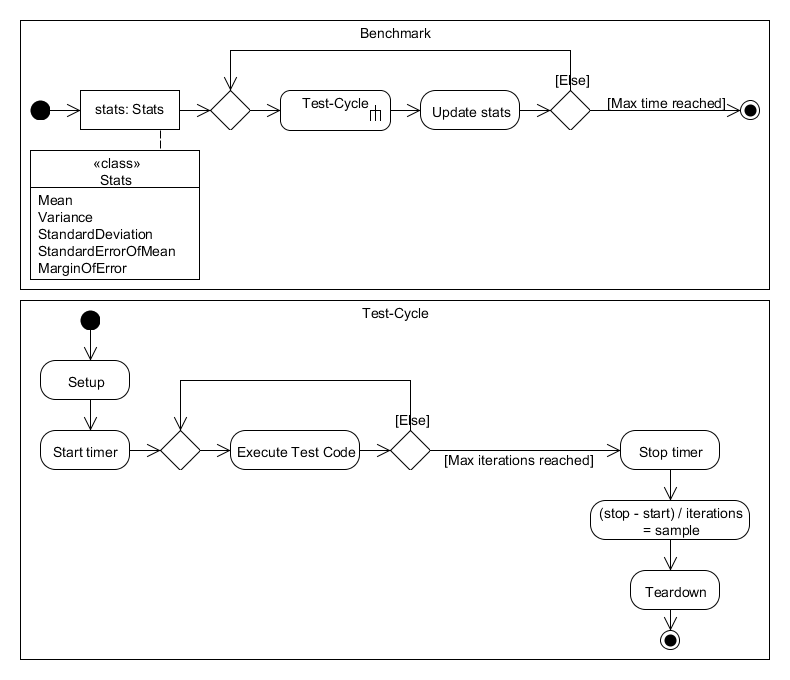
\includegraphics[scale=0.5]{Bilder/BenchmarkJS.png}
	\caption{BenchmarkJS Benchmark Prozess\cite{BenchmarkJSHowItWorks}}
	\label{bmjs-benchmark-prozess}
\end{figure}
Innerhalb jedes Test-Zyklus wird der zu testende Code in einer Schleife durchlaufen. Vor der Codeausführung findet eine Setup-Phase zur Initialisierung des Tests und im Anschluss eine Teardown-Phase zum Aufräumen des Tests statt. Das Ergebnis eines Test-Zyklus ist ein sogenanntes Sample. Das Sample berechnet sich durch die Formel $ \frac{Ende - Start}{Iterationen} $. Die Anzahl der Iterationen wird von BenchmarkJS dynamisch angepasst. Nach jedem Test-Zyklus wird das Sample in einer Liste gespeichert, um anschließend statistische Werte auf Basis dieser Liste zu berechnen (Anhang 2) \cite{BenchmarkJSQuelltext}\cite{UncertaintyCalculations}. Abbildung \ref{bmjs-benchmark-prozess} zeigt schematisch den Ablauf von BenchmarkJS. Durch die Berechnung des Durchschnitts und der Standard-Abweichung aller Samples ergibt sich der relative Fehler mittels einer T-Verteilung \cite[S. 440ff.]{Papula2001}. Ist dieser relative Fehler größer als 1\%, erhöht BenchmarkJS die Anzahl der Iterationen in einem Test-Zyklus, um bessere Ergebnisse zu erzielen \cite{BenchmarkJSQuelltext}. Störungen durch Hintergrundprozesse fallen dadurch weniger ins Gewicht. 
\begin{lstlisting}[caption={BenchmarkJS synchrone Benchmarks}\label{BenchmarkJSSynchron}]
// Synchrone Implementierung
var bench = new Benchmark('', {
	'fn': function() {
		// Test code
	},
	'onComplete': function() {
		var meanInMs = this.stats.mean * 1000;
	}
});
bench.run();
\end{lstlisting}
In den folgenden Kapiteln werden zum Teil sehr unterschiedliche Implementierungen durch Zeitmessungen untersucht. Diese Implementierungen unterscheiden sich durch Asynchrones- und Synchrones-Verhalten. Für beide Varianten bietet BenchmarkJS eine Schnittstelle an. Listing \ref{BenchmarkJSSynchron} und \ref{BenchmarkJSAsynchron} zeigen jeweils die Verwendung von BenchmarkJS für einen synchronen und einen asynchronen Vorgang. Der asynchrone Vorgang unterscheidet sich dadurch, dass BenchmarkJS das Ende der Codeausführung nicht selbst feststellen kann. Aus diesem Grund muss bei der asynchronen Variante nach der Codeausführung ein \gls{Promise} abgeschlossen werden. Somit lassen sich alle in den folgenden Kapiteln durchgeführten Tests hinsichtlich ihrer Performance messen. 
\begin{lstlisting}[caption={BenchmarkJS asynchrone Benchmarks}\label{BenchmarkJSAsynchron}]
// Asynchrone implementierung
var bench = new Benchmark('', {
	'defer': true,
	'fn': function(deferred) {
		doAsyncWork(function(){
		// Benchrichtigt BenchmarkJS darüber,
		// dass der Durchlauf fertig ist.
			deferred.resolve();
		});
	},
	'onComplete': function() {
		var meanInMs = this.stats.mean * 1000;
	}
});
bench.run();
\end{lstlisting}
